% Options for packages loaded elsewhere
\PassOptionsToPackage{unicode}{hyperref}
\PassOptionsToPackage{hyphens}{url}
\PassOptionsToPackage{dvipsnames,svgnames,x11names}{xcolor}
%
\documentclass[
  letterpaper,
  DIV=11,
  numbers=noendperiod]{scrreprt}

\usepackage{amsmath,amssymb}
\usepackage{iftex}
\ifPDFTeX
  \usepackage[T1]{fontenc}
  \usepackage[utf8]{inputenc}
  \usepackage{textcomp} % provide euro and other symbols
\else % if luatex or xetex
  \usepackage{unicode-math}
  \defaultfontfeatures{Scale=MatchLowercase}
  \defaultfontfeatures[\rmfamily]{Ligatures=TeX,Scale=1}
\fi
\usepackage{lmodern}
\ifPDFTeX\else  
    % xetex/luatex font selection
\fi
% Use upquote if available, for straight quotes in verbatim environments
\IfFileExists{upquote.sty}{\usepackage{upquote}}{}
\IfFileExists{microtype.sty}{% use microtype if available
  \usepackage[]{microtype}
  \UseMicrotypeSet[protrusion]{basicmath} % disable protrusion for tt fonts
}{}
\makeatletter
\@ifundefined{KOMAClassName}{% if non-KOMA class
  \IfFileExists{parskip.sty}{%
    \usepackage{parskip}
  }{% else
    \setlength{\parindent}{0pt}
    \setlength{\parskip}{6pt plus 2pt minus 1pt}}
}{% if KOMA class
  \KOMAoptions{parskip=half}}
\makeatother
\usepackage{xcolor}
\setlength{\emergencystretch}{3em} % prevent overfull lines
\setcounter{secnumdepth}{5}
% Make \paragraph and \subparagraph free-standing
\ifx\paragraph\undefined\else
  \let\oldparagraph\paragraph
  \renewcommand{\paragraph}[1]{\oldparagraph{#1}\mbox{}}
\fi
\ifx\subparagraph\undefined\else
  \let\oldsubparagraph\subparagraph
  \renewcommand{\subparagraph}[1]{\oldsubparagraph{#1}\mbox{}}
\fi

\usepackage{color}
\usepackage{fancyvrb}
\newcommand{\VerbBar}{|}
\newcommand{\VERB}{\Verb[commandchars=\\\{\}]}
\DefineVerbatimEnvironment{Highlighting}{Verbatim}{commandchars=\\\{\}}
% Add ',fontsize=\small' for more characters per line
\usepackage{framed}
\definecolor{shadecolor}{RGB}{241,243,245}
\newenvironment{Shaded}{\begin{snugshade}}{\end{snugshade}}
\newcommand{\AlertTok}[1]{\textcolor[rgb]{0.68,0.00,0.00}{#1}}
\newcommand{\AnnotationTok}[1]{\textcolor[rgb]{0.37,0.37,0.37}{#1}}
\newcommand{\AttributeTok}[1]{\textcolor[rgb]{0.40,0.45,0.13}{#1}}
\newcommand{\BaseNTok}[1]{\textcolor[rgb]{0.68,0.00,0.00}{#1}}
\newcommand{\BuiltInTok}[1]{\textcolor[rgb]{0.00,0.23,0.31}{#1}}
\newcommand{\CharTok}[1]{\textcolor[rgb]{0.13,0.47,0.30}{#1}}
\newcommand{\CommentTok}[1]{\textcolor[rgb]{0.37,0.37,0.37}{#1}}
\newcommand{\CommentVarTok}[1]{\textcolor[rgb]{0.37,0.37,0.37}{\textit{#1}}}
\newcommand{\ConstantTok}[1]{\textcolor[rgb]{0.56,0.35,0.01}{#1}}
\newcommand{\ControlFlowTok}[1]{\textcolor[rgb]{0.00,0.23,0.31}{#1}}
\newcommand{\DataTypeTok}[1]{\textcolor[rgb]{0.68,0.00,0.00}{#1}}
\newcommand{\DecValTok}[1]{\textcolor[rgb]{0.68,0.00,0.00}{#1}}
\newcommand{\DocumentationTok}[1]{\textcolor[rgb]{0.37,0.37,0.37}{\textit{#1}}}
\newcommand{\ErrorTok}[1]{\textcolor[rgb]{0.68,0.00,0.00}{#1}}
\newcommand{\ExtensionTok}[1]{\textcolor[rgb]{0.00,0.23,0.31}{#1}}
\newcommand{\FloatTok}[1]{\textcolor[rgb]{0.68,0.00,0.00}{#1}}
\newcommand{\FunctionTok}[1]{\textcolor[rgb]{0.28,0.35,0.67}{#1}}
\newcommand{\ImportTok}[1]{\textcolor[rgb]{0.00,0.46,0.62}{#1}}
\newcommand{\InformationTok}[1]{\textcolor[rgb]{0.37,0.37,0.37}{#1}}
\newcommand{\KeywordTok}[1]{\textcolor[rgb]{0.00,0.23,0.31}{#1}}
\newcommand{\NormalTok}[1]{\textcolor[rgb]{0.00,0.23,0.31}{#1}}
\newcommand{\OperatorTok}[1]{\textcolor[rgb]{0.37,0.37,0.37}{#1}}
\newcommand{\OtherTok}[1]{\textcolor[rgb]{0.00,0.23,0.31}{#1}}
\newcommand{\PreprocessorTok}[1]{\textcolor[rgb]{0.68,0.00,0.00}{#1}}
\newcommand{\RegionMarkerTok}[1]{\textcolor[rgb]{0.00,0.23,0.31}{#1}}
\newcommand{\SpecialCharTok}[1]{\textcolor[rgb]{0.37,0.37,0.37}{#1}}
\newcommand{\SpecialStringTok}[1]{\textcolor[rgb]{0.13,0.47,0.30}{#1}}
\newcommand{\StringTok}[1]{\textcolor[rgb]{0.13,0.47,0.30}{#1}}
\newcommand{\VariableTok}[1]{\textcolor[rgb]{0.07,0.07,0.07}{#1}}
\newcommand{\VerbatimStringTok}[1]{\textcolor[rgb]{0.13,0.47,0.30}{#1}}
\newcommand{\WarningTok}[1]{\textcolor[rgb]{0.37,0.37,0.37}{\textit{#1}}}

\providecommand{\tightlist}{%
  \setlength{\itemsep}{0pt}\setlength{\parskip}{0pt}}\usepackage{longtable,booktabs,array}
\usepackage{calc} % for calculating minipage widths
% Correct order of tables after \paragraph or \subparagraph
\usepackage{etoolbox}
\makeatletter
\patchcmd\longtable{\par}{\if@noskipsec\mbox{}\fi\par}{}{}
\makeatother
% Allow footnotes in longtable head/foot
\IfFileExists{footnotehyper.sty}{\usepackage{footnotehyper}}{\usepackage{footnote}}
\makesavenoteenv{longtable}
\usepackage{graphicx}
\makeatletter
\def\maxwidth{\ifdim\Gin@nat@width>\linewidth\linewidth\else\Gin@nat@width\fi}
\def\maxheight{\ifdim\Gin@nat@height>\textheight\textheight\else\Gin@nat@height\fi}
\makeatother
% Scale images if necessary, so that they will not overflow the page
% margins by default, and it is still possible to overwrite the defaults
% using explicit options in \includegraphics[width, height, ...]{}
\setkeys{Gin}{width=\maxwidth,height=\maxheight,keepaspectratio}
% Set default figure placement to htbp
\makeatletter
\def\fps@figure{htbp}
\makeatother

\KOMAoption{captions}{tableheading}
\makeatletter
\@ifpackageloaded{tcolorbox}{}{\usepackage[skins,breakable]{tcolorbox}}
\@ifpackageloaded{fontawesome5}{}{\usepackage{fontawesome5}}
\definecolor{quarto-callout-color}{HTML}{909090}
\definecolor{quarto-callout-note-color}{HTML}{0758E5}
\definecolor{quarto-callout-important-color}{HTML}{CC1914}
\definecolor{quarto-callout-warning-color}{HTML}{EB9113}
\definecolor{quarto-callout-tip-color}{HTML}{00A047}
\definecolor{quarto-callout-caution-color}{HTML}{FC5300}
\definecolor{quarto-callout-color-frame}{HTML}{acacac}
\definecolor{quarto-callout-note-color-frame}{HTML}{4582ec}
\definecolor{quarto-callout-important-color-frame}{HTML}{d9534f}
\definecolor{quarto-callout-warning-color-frame}{HTML}{f0ad4e}
\definecolor{quarto-callout-tip-color-frame}{HTML}{02b875}
\definecolor{quarto-callout-caution-color-frame}{HTML}{fd7e14}
\makeatother
\makeatletter
\makeatother
\makeatletter
\makeatother
\makeatletter
\@ifpackageloaded{caption}{}{\usepackage{caption}}
\AtBeginDocument{%
\ifdefined\contentsname
  \renewcommand*\contentsname{Table of contents}
\else
  \newcommand\contentsname{Table of contents}
\fi
\ifdefined\listfigurename
  \renewcommand*\listfigurename{List of Figures}
\else
  \newcommand\listfigurename{List of Figures}
\fi
\ifdefined\listtablename
  \renewcommand*\listtablename{List of Tables}
\else
  \newcommand\listtablename{List of Tables}
\fi
\ifdefined\figurename
  \renewcommand*\figurename{Figure}
\else
  \newcommand\figurename{Figure}
\fi
\ifdefined\tablename
  \renewcommand*\tablename{Table}
\else
  \newcommand\tablename{Table}
\fi
}
\@ifpackageloaded{float}{}{\usepackage{float}}
\floatstyle{ruled}
\@ifundefined{c@chapter}{\newfloat{codelisting}{h}{lop}}{\newfloat{codelisting}{h}{lop}[chapter]}
\floatname{codelisting}{Listing}
\newcommand*\listoflistings{\listof{codelisting}{List of Listings}}
\makeatother
\makeatletter
\@ifpackageloaded{caption}{}{\usepackage{caption}}
\@ifpackageloaded{subcaption}{}{\usepackage{subcaption}}
\makeatother
\makeatletter
\@ifpackageloaded{tcolorbox}{}{\usepackage[skins,breakable]{tcolorbox}}
\makeatother
\makeatletter
\@ifundefined{shadecolor}{\definecolor{shadecolor}{rgb}{.97, .97, .97}}
\makeatother
\makeatletter
\makeatother
\makeatletter
\makeatother
\ifLuaTeX
  \usepackage{selnolig}  % disable illegal ligatures
\fi
\usepackage[]{biblatex}
\addbibresource{references.bib}
\IfFileExists{bookmark.sty}{\usepackage{bookmark}}{\usepackage{hyperref}}
\IfFileExists{xurl.sty}{\usepackage{xurl}}{} % add URL line breaks if available
\urlstyle{same} % disable monospaced font for URLs
\hypersetup{
  pdftitle={Chapter 0 R quarto and Tidy data},
  colorlinks=true,
  linkcolor={blue},
  filecolor={Maroon},
  citecolor={Blue},
  urlcolor={Blue},
  pdfcreator={LaTeX via pandoc}}

\title{Chapter 0 R quarto and Tidy data}
\author{}
\date{}

\begin{document}
\maketitle
\ifdefined\Shaded\renewenvironment{Shaded}{\begin{tcolorbox}[frame hidden, breakable, interior hidden, sharp corners, borderline west={3pt}{0pt}{shadecolor}, boxrule=0pt, enhanced]}{\end{tcolorbox}}\fi

\renewcommand*\contentsname{Table of contents}
{
\hypersetup{linkcolor=}
\setcounter{tocdepth}{2}
\tableofcontents
}
\hypertarget{installing-r-and-rstudio}{%
\chapter{\texorpdfstring{Installing \texttt{R} and
RStudio}{Installing R and RStudio}}\label{installing-r-and-rstudio}}

In this course, we will be using R \url{https://www.r-project.org/}, an
open-source (i.e., free) software package for data analysis. This
software is available for essentially all computing platforms
(e.g.~Windows, Linux, Unix, Mac) is maintained and developed by a huge
community of users including many of the world's foremost statisticians.

R is a programming language but you may not be required to do a lot of
programming for your course work. R includes functions which enables us
to perform a full range of statistical analyses.

\textbf{For installing R software, please visit
\url{https://cran.stat.auckland.ac.nz/} and follow the instructions.}

Note that the R software will be sitting in the background in RStudio
and you will not be using the standalone version of R in this course.

RStudio \url{https://www.rstudio.com/products/rstudio/} is an integrated
development environment (IDE) for R. It includes a console and a
sophisticated code editor. It also contains tools for plotting, history,
debugging, and management of workspaces and projects. RStudio has many
other features such as authoring HTML, PDF, Word Documents, and slide
shows. In order to download RStudio (Desktop edition, open source), go
to

\url{https://www.rstudio.com/products/rstudio/download/}

Download the installation file and run it. \textbf{Note that RStudio
must be installed after installing R.}

R/RStudio can also be run on a cloud platform at
\url{https://rstudio.cloud/} after creating a \emph{free} account. Be
aware though that some of the packages covered in this course may not
work in the cloud platform and there is a maximum amount of computing
time. We \emph{do not recommend} relying on the cloud platform for this
course.

If you open RStudio, you will see something similar to the screen shot
shown in Figure~\ref{fig-rstud}:

\begin{figure}

{\centering 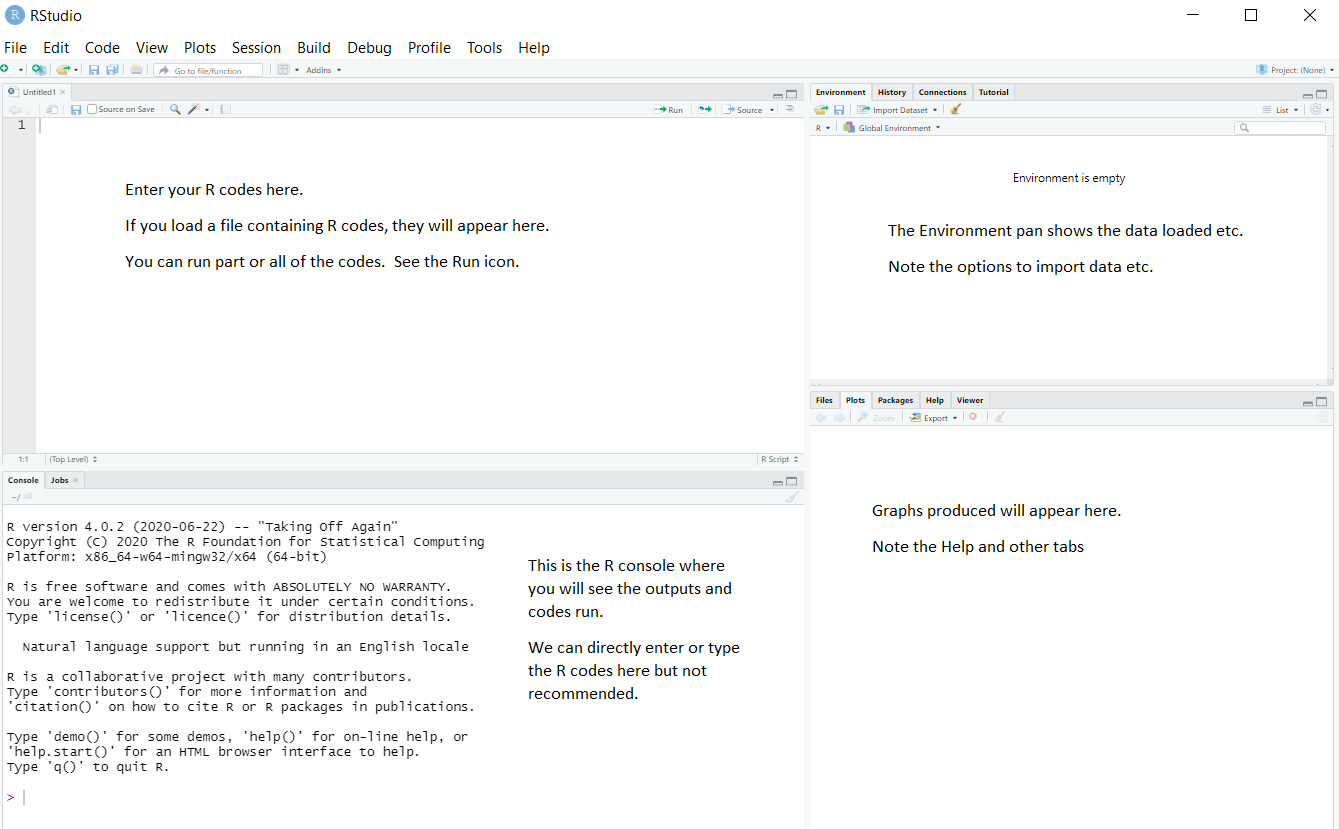
\includegraphics{img/Rstudio.png}

}

\caption{\label{fig-rstud}An RStudio window}

\end{figure}

RStudio has many options, such as uploading files to a server, creating
documents, etc. You will be using only a few of the options. You will
\emph{not} be using the menus such as \emph{Build}, \emph{Debug},
\emph{Profile} at all in this course.

You can either type or copy and paste the R codes appearing in this
section on to the R Script window and run them.

\hypertarget{quarto}{%
\chapter*{Quarto}\label{quarto}}
\addcontentsline{toc}{chapter}{Quarto}

This course will be using \href{https://quarto.org/}{Quarto}
\texttt{*.qmd} files rather than raw \texttt{*.R} files. Heard of
Rmarkdown? Well, Quarto is the successor to Rmarkdown. So, if you're
just starting to use R, then you should begin with Quarto rather than
Rmarkdown, because most/all new development will be going into Quarto.

Here's some information to get you started:
\url{https://quarto.org/docs/get-started/hello/rstudio.html}.

And some other useful tips: \url{https://r4ds.hadley.nz/quarto}.

We will be using Quarto documents. You can open a blank one by clicking
File \textgreater{} New File \textgreater{} Quarto Document.

You can then make your own document or copy code from the course website
and paste it into your new Quarto file.

\hypertarget{including-text-and-code}{%
\chapter{Including text and code}\label{including-text-and-code}}

The one advantage of Quarto (and its predecessor R markdown) is being
able to include general text along side code chunks.

You can insert a code chunk using the green button near the top right of
your quarto document window.

\hypertarget{setting-up-a-quarto-project}{%
\chapter{Setting up a Quarto
project}\label{setting-up-a-quarto-project}}

It is a good idea to get into the habit of using Quarto projects, rather
than just R scripts. Here is a step-by-step guide to creating a project
for your workshops. You don't have to use projects, but they are very
useful.

\begin{enumerate}
\def\labelenumi{\arabic{enumi}.}
\tightlist
\item
  Open RStudio. (Optional: click on the little window symbol at the top
  and select ``Console on Right'')
\end{enumerate}

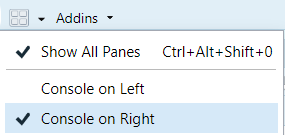
\includegraphics{img/console_right.png}

\begin{enumerate}
\def\labelenumi{\arabic{enumi}.}
\setcounter{enumi}{1}
\item
  If you haven't already, make a directory on your computer where you
  want to keep your code for this course.
\item
  Make a new project. Select the ``Project'' button at the top-right of
  Rstudio, and select ``New Project\ldots{}''.
\end{enumerate}

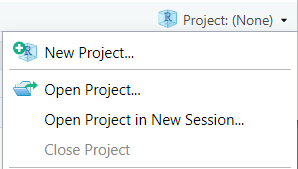
\includegraphics{img/open_project.png}

\begin{enumerate}
\def\labelenumi{\arabic{enumi}.}
\setcounter{enumi}{3}
\tightlist
\item
  In the pop-up window:
\end{enumerate}

\begin{itemize}
\tightlist
\item
  Select ``New Directory''
\end{itemize}

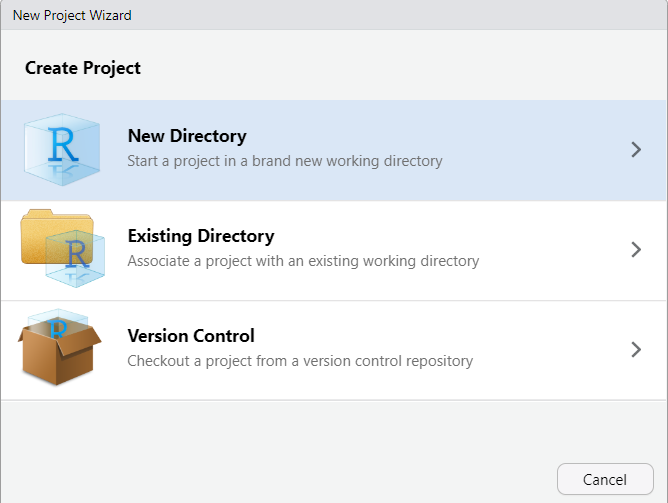
\includegraphics{img/new_direct.png}

\begin{itemize}
\tightlist
\item
  Select ``Quarto Project''
\end{itemize}

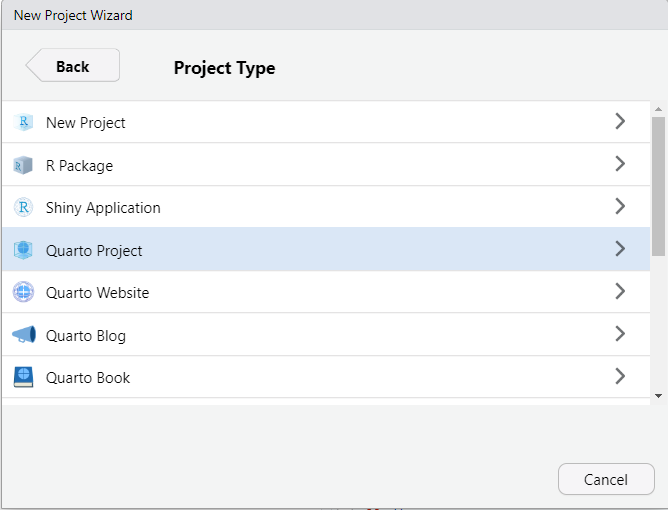
\includegraphics{img/quarto_proj.png}

\begin{itemize}
\tightlist
\item
  Choose your directory via the ``Browse'', and then give the project a
  name like ``161250\_workshops''
\end{itemize}

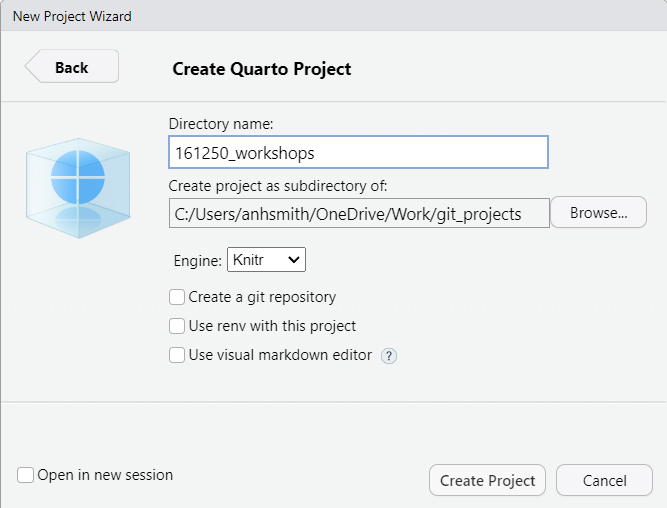
\includegraphics{img/dir_name.png}

\begin{itemize}
\tightlist
\item
  Finish by clicking on ``Create Project''.
\end{itemize}

The project should now be created, and you'll likely have an open *.qmd
file (something like ``161250\_workshops.qmd'') in the top-right window
of Rstudio. We want to make a *.qmd file for this workshop.

\begin{enumerate}
\def\labelenumi{\arabic{enumi}.}
\setcounter{enumi}{4}
\tightlist
\item
  Right-click on the qmd tab and select ``Rename'', and rename it
  ``workshop2.qmd'' or something similar. (Alternatively, just make a
  new file via the menus: \emph{File \textgreater{} New File
  \textgreater{} Quarto Document}.)
\end{enumerate}

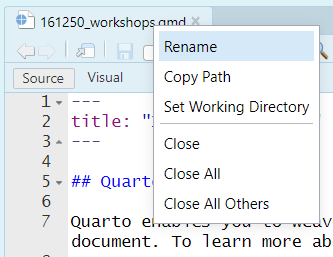
\includegraphics{img/rename_qmd.png}

Now you have a document for your Workshop work. You can:

\begin{itemize}
\tightlist
\item
  Write headings with lines beginning with ``\#''.
\item
  Write text in the main part of the document.
\item
  Make a code chunk for your R code using \emph{Ctrl-Alt-i}. Write R
  code in the code chunks.
\end{itemize}

Like so:

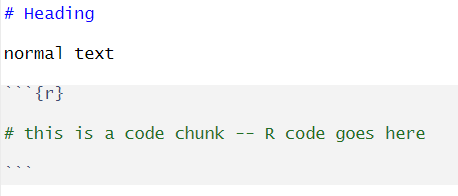
\includegraphics{img/chunk.png}

There are lots of tutorials online covering the basics of Quarto, and
we'll discuss them during our own workshops. Here are a couple for
starters:

\url{https://quarto.org/docs/get-started/hello/rstudio.html}

\url{https://www.youtube.com/watch?v=c654j7aQjcg}

There are many advantages of Quarto projects. One is that you can put
datasets into the project folder, and they'll be easily accessible
within your project, without having to worry about file paths.

You can easily open a recent past projects via the ``Projects'' button
on the top-right of Rstudio.

This covers some introduces tidyverse and some functions we will be
using in this course. This is not meant to be an exhaustive list and
students are encourage to read R4 data science or other free tutorials
online.

\hypertarget{definitions}{%
\chapter{Definitions}\label{definitions}}

Before we talk more about data it is useful to define some terms:

\begin{itemize}
\item
  A \emph{variable} is a quantity, quality, or property that you can
  measure.
\item
  A \emph{value} is the state of a variable when you measure it. The
  value of a variable may change from measurement to measurement.
\item
  An \emph{observation} is a set of measurements made under similar
  conditions (you usually make all of the measurements in an observation
  at the same time and on the same object). An observation will contain
  several values, each associated with a different variable. We'll
  sometimes refer to an observation as a data point.
\item
  \emph{Tabular data} is a set of values, each associated with a
  variable and an observation. Tabular data is tidy if each value is
  placed in its own ``cell'', each variable in its own column, and each
  observation in its own row.
\end{itemize}

\hypertarget{introduction-to-the-tidyverse}{%
\chapter{Introduction to the
tidyverse}\label{introduction-to-the-tidyverse}}

We will be largely using the \texttt{tidyverse} suite of packages for
data organisation, summarising, and plotting; see
\url{https://www.tidyverse.org/}.

Let's load that package now:

\begin{Shaded}
\begin{Highlighting}[]
\FunctionTok{library}\NormalTok{(tidyverse)}
\end{Highlighting}
\end{Shaded}

Recommended reading to accompany this workshop is pages 1-11 of R for
Data Science \url{https://r4ds.hadley.nz/}

\hypertarget{tidy-data}{%
\chapter{Tidy data}\label{tidy-data}}

There are three interrelated rules that make a dataset tidy:

\begin{itemize}
\tightlist
\item
  Each variable is a column; each column is a variable.
\item
  Each observation is a row; each row is an observation.
\item
  Each value is a cell; each cell is a single value.
\end{itemize}

\begin{figure}

{\centering 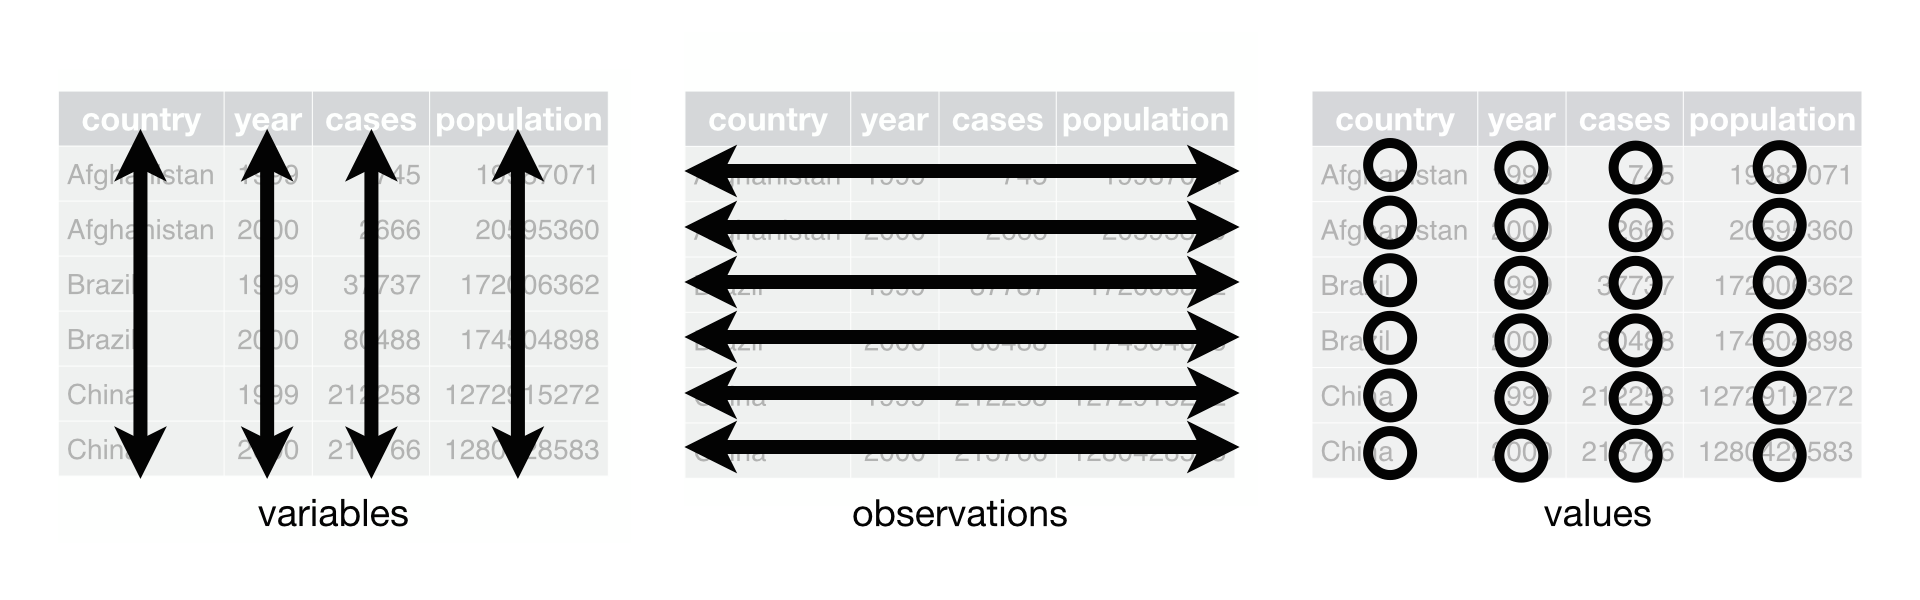
\includegraphics{images/tidy_data.png}

}

\caption{\label{fig-tidy}Tidy data}

\end{figure}

Why ensure that your data is tidy? There are two main advantages:

\begin{itemize}
\item
  There's a general advantage to picking one consistent way of storing
  data. If you have a consistent data structure, it's easier to learn
  the tools that work with it because they have an underlying
  uniformity.
\item
  There's a specific advantage to placing variables in columns because
  it allows R's vectorized nature to shine. Most built-in R functions
  work with vectors of values.
\end{itemize}

dplyr, ggplot2, and all the other packages in the tidyverse are designed
to work with tidy data.

\hypertarget{summarize-data}{%
\chapter{Summarize data}\label{summarize-data}}

Apply summary functions to columns to create a new table of summary
statistics. Summary functions take vectors as input and return one value
back.

\begin{itemize}
\tightlist
\item
  \texttt{summarize(.data,\ ..\ )} : Compute table of summaries
\end{itemize}

\begin{Shaded}
\begin{Highlighting}[]
\NormalTok{mtcars }\SpecialCharTok{|\textgreater{}} \FunctionTok{summarize}\NormalTok{(}\AttributeTok{avg =} \FunctionTok{mean}\NormalTok{(mpg))}
\end{Highlighting}
\end{Shaded}

\begin{verbatim}
       avg
1 20.09062
\end{verbatim}

\begin{itemize}
\tightlist
\item
  \texttt{count(.data,\ ...,\ wt\ =\ NULL,\ sort\ =\ FLASE,\ name\ =\ NULL)}:
  Count number of rows in each group defined by the variables in \ldots.
  Also \texttt{tally()}, \texttt{add\_count()}, and
  \texttt{add\_tally()}.
\end{itemize}

\begin{Shaded}
\begin{Highlighting}[]
\NormalTok{mtcars }\SpecialCharTok{|\textgreater{}} \FunctionTok{count}\NormalTok{(cyl)}
\end{Highlighting}
\end{Shaded}

\begin{verbatim}
  cyl  n
1   4 11
2   6  7
3   8 14
\end{verbatim}

\hypertarget{group-cases}{%
\chapter{Group Cases}\label{group-cases}}

\begin{itemize}
\tightlist
\item
  Use \texttt{group\_by(.data,\ ...,\ .add\ =\ FALSE,\ .drop\ =\ TRUE)}
  to created a ``grouped'' copy of a table grouped by columns in \ldots.
  dplyr functions will manipulate each ``group'' separately and combine
  the results.
\end{itemize}

\begin{Shaded}
\begin{Highlighting}[]
\NormalTok{mtcars }\SpecialCharTok{|\textgreater{}}
  \FunctionTok{group\_by}\NormalTok{(cyl) }\SpecialCharTok{|\textgreater{}}
  \FunctionTok{summarize}\NormalTok{(}\AttributeTok{avg =} \FunctionTok{mean}\NormalTok{(mpg))}
\end{Highlighting}
\end{Shaded}

\begin{verbatim}
# A tibble: 3 x 2
    cyl   avg
  <dbl> <dbl>
1     4  26.7
2     6  19.7
3     8  15.1
\end{verbatim}

\hypertarget{extract-cases}{%
\chapter{Extract cases}\label{extract-cases}}

\begin{itemize}
\tightlist
\item
  \texttt{filter(.data,\ ...,\ .preserve\ =\ FALSE)}: Extract rows that
  meet logical criteria.
\end{itemize}

\begin{Shaded}
\begin{Highlighting}[]
\NormalTok{mtcars }\SpecialCharTok{|\textgreater{}} \FunctionTok{filter}\NormalTok{(mpg }\SpecialCharTok{\textgreater{}} \DecValTok{20}\NormalTok{)}
\end{Highlighting}
\end{Shaded}

\begin{verbatim}
                mpg cyl  disp  hp drat    wt  qsec vs am gear carb
Mazda RX4      21.0   6 160.0 110 3.90 2.620 16.46  0  1    4    4
Mazda RX4 Wag  21.0   6 160.0 110 3.90 2.875 17.02  0  1    4    4
Datsun 710     22.8   4 108.0  93 3.85 2.320 18.61  1  1    4    1
Hornet 4 Drive 21.4   6 258.0 110 3.08 3.215 19.44  1  0    3    1
Merc 240D      24.4   4 146.7  62 3.69 3.190 20.00  1  0    4    2
Merc 230       22.8   4 140.8  95 3.92 3.150 22.90  1  0    4    2
Fiat 128       32.4   4  78.7  66 4.08 2.200 19.47  1  1    4    1
Honda Civic    30.4   4  75.7  52 4.93 1.615 18.52  1  1    4    2
Toyota Corolla 33.9   4  71.1  65 4.22 1.835 19.90  1  1    4    1
Toyota Corona  21.5   4 120.1  97 3.70 2.465 20.01  1  0    3    1
Fiat X1-9      27.3   4  79.0  66 4.08 1.935 18.90  1  1    4    1
Porsche 914-2  26.0   4 120.3  91 4.43 2.140 16.70  0  1    5    2
Lotus Europa   30.4   4  95.1 113 3.77 1.513 16.90  1  1    5    2
Volvo 142E     21.4   4 121.0 109 4.11 2.780 18.60  1  1    4    2
\end{verbatim}

Logical and boolean operations to use with filter() - \texttt{==},
\texttt{!=} - \texttt{\textless{}}, \texttt{\textgreater{}} -
\texttt{\textless{}=}, \texttt{\textgreater{}=} - \texttt{is.na()},
\texttt{!is.na()} - \texttt{\%in\%} - \texttt{\textbar{}} See
\texttt{?base::Logic} and \texttt{?Comparison} for help.

\begin{itemize}
\tightlist
\item
  \texttt{distinct(.data,\ ...,\ .keep\_all\ =\ FALSE)}: Remove rows
  with duplicate values.
\end{itemize}

\begin{Shaded}
\begin{Highlighting}[]
\NormalTok{mtcars }\SpecialCharTok{|\textgreater{}} \FunctionTok{distinct}\NormalTok{(gear)}
\end{Highlighting}
\end{Shaded}

\begin{verbatim}
               gear
Mazda RX4         4
Hornet 4 Drive    3
Porsche 914-2     5
\end{verbatim}

\begin{itemize}
\tightlist
\item
  \texttt{pull(.data,\ var\ =\ -1,\ name\ =\ NULL,\ ...)}: Extract
  column values as a vector, by name or index.
\end{itemize}

\begin{Shaded}
\begin{Highlighting}[]
\NormalTok{mtcars }\SpecialCharTok{|\textgreater{}} \FunctionTok{pull}\NormalTok{(wt)}
\end{Highlighting}
\end{Shaded}

\begin{verbatim}
 [1] 2.620 2.875 2.320 3.215 3.440 3.460 3.570 3.190 3.150 3.440 3.440 4.070
[13] 3.730 3.780 5.250 5.424 5.345 2.200 1.615 1.835 2.465 3.520 3.435 3.840
[25] 3.845 1.935 2.140 1.513 3.170 2.770 3.570 2.780
\end{verbatim}

\begin{itemize}
\tightlist
\item
  \texttt{select(.data,\ ...)}: Extract columns as a table.
\end{itemize}

\begin{Shaded}
\begin{Highlighting}[]
\NormalTok{mtcars }\SpecialCharTok{|\textgreater{}} \FunctionTok{select}\NormalTok{(mpg, wt)}
\end{Highlighting}
\end{Shaded}

\begin{verbatim}
                     mpg    wt
Mazda RX4           21.0 2.620
Mazda RX4 Wag       21.0 2.875
Datsun 710          22.8 2.320
Hornet 4 Drive      21.4 3.215
Hornet Sportabout   18.7 3.440
Valiant             18.1 3.460
Duster 360          14.3 3.570
Merc 240D           24.4 3.190
Merc 230            22.8 3.150
Merc 280            19.2 3.440
Merc 280C           17.8 3.440
Merc 450SE          16.4 4.070
Merc 450SL          17.3 3.730
Merc 450SLC         15.2 3.780
Cadillac Fleetwood  10.4 5.250
Lincoln Continental 10.4 5.424
Chrysler Imperial   14.7 5.345
Fiat 128            32.4 2.200
Honda Civic         30.4 1.615
Toyota Corolla      33.9 1.835
Toyota Corona       21.5 2.465
Dodge Challenger    15.5 3.520
AMC Javelin         15.2 3.435
Camaro Z28          13.3 3.840
Pontiac Firebird    19.2 3.845
Fiat X1-9           27.3 1.935
Porsche 914-2       26.0 2.140
Lotus Europa        30.4 1.513
Ford Pantera L      15.8 3.170
Ferrari Dino        19.7 2.770
Maserati Bora       15.0 3.570
Volvo 142E          21.4 2.780
\end{verbatim}

Use these helpers with select() - \texttt{contains(match)} -
\texttt{num\_range(prefix,\ range)} - \texttt{:}, e.g., \texttt{mpg:cyl}
- \texttt{ends\_with(match)} - \texttt{all\_of(x)} or
\texttt{any\_of(x,\ ...,\ vars)} - \texttt{!}, e.g., \texttt{!gear} -
\texttt{starts\_with(match)} - \texttt{matches(match)} -
\texttt{everything()}

\begin{itemize}
\tightlist
\item
  \texttt{dplyr::case\_when()}: multi-case if\_else()
\end{itemize}

\begin{Shaded}
\begin{Highlighting}[]
\NormalTok{starwars }\SpecialCharTok{|\textgreater{}}
  \FunctionTok{mutate}\NormalTok{(}\AttributeTok{type =} \FunctionTok{case\_when}\NormalTok{(}
\NormalTok{    height }\SpecialCharTok{\textgreater{}} \DecValTok{200} \SpecialCharTok{|}\NormalTok{ mass }\SpecialCharTok{\textgreater{}} \DecValTok{200} \SpecialCharTok{\textasciitilde{}} \StringTok{"large"}\NormalTok{,}
\NormalTok{    species }\SpecialCharTok{==} \StringTok{"Droid"} \SpecialCharTok{\textasciitilde{}} \StringTok{"robot"}\NormalTok{,}
    \ConstantTok{TRUE} \SpecialCharTok{\textasciitilde{}} \StringTok{"other"}
\NormalTok{  ))}
\end{Highlighting}
\end{Shaded}

\begin{verbatim}
# A tibble: 87 x 15
   name     height  mass hair_color skin_color eye_color birth_year sex   gender
   <chr>     <int> <dbl> <chr>      <chr>      <chr>          <dbl> <chr> <chr> 
 1 Luke Sk~    172    77 blond      fair       blue            19   male  mascu~
 2 C-3PO       167    75 <NA>       gold       yellow         112   none  mascu~
 3 R2-D2        96    32 <NA>       white, bl~ red             33   none  mascu~
 4 Darth V~    202   136 none       white      yellow          41.9 male  mascu~
 5 Leia Or~    150    49 brown      light      brown           19   fema~ femin~
 6 Owen La~    178   120 brown, gr~ light      blue            52   male  mascu~
 7 Beru Wh~    165    75 brown      light      blue            47   fema~ femin~
 8 R5-D4        97    32 <NA>       white, red red             NA   none  mascu~
 9 Biggs D~    183    84 black      light      brown           24   male  mascu~
10 Obi-Wan~    182    77 auburn, w~ fair       blue-gray       57   male  mascu~
# i 77 more rows
# i 6 more variables: homeworld <chr>, species <chr>, films <list>,
#   vehicles <list>, starships <list>, type <chr>
\end{verbatim}

\hypertarget{alter-data}{%
\chapter{Alter data}\label{alter-data}}

\begin{Shaded}
\begin{Highlighting}[]
\NormalTok{df }\OtherTok{\textless{}{-}} \FunctionTok{tibble}\NormalTok{(}\AttributeTok{x\_1 =} \FunctionTok{c}\NormalTok{(}\DecValTok{1}\NormalTok{, }\DecValTok{2}\NormalTok{), }\AttributeTok{x\_2 =} \FunctionTok{c}\NormalTok{(}\DecValTok{3}\NormalTok{, }\DecValTok{4}\NormalTok{), }\AttributeTok{y =} \FunctionTok{c}\NormalTok{(}\DecValTok{4}\NormalTok{, }\DecValTok{5}\NormalTok{))}
\end{Highlighting}
\end{Shaded}

\begin{itemize}
\tightlist
\item
  \texttt{across(.cols,\ .fun,\ ...,\ .name\ =\ NULL)}: summarize or
  mutate multiple columns in the same way.
\end{itemize}

\begin{Shaded}
\begin{Highlighting}[]
\NormalTok{df }\SpecialCharTok{|\textgreater{}} \FunctionTok{summarize}\NormalTok{(}\FunctionTok{across}\NormalTok{(}\FunctionTok{everything}\NormalTok{(), mean))}
\end{Highlighting}
\end{Shaded}

\begin{verbatim}
# A tibble: 1 x 3
    x_1   x_2     y
  <dbl> <dbl> <dbl>
1   1.5   3.5   4.5
\end{verbatim}

\begin{itemize}
\tightlist
\item
  \texttt{c\_across(.cols)}: Compute across columns in row-wise data.
\end{itemize}

\begin{Shaded}
\begin{Highlighting}[]
\NormalTok{df }\SpecialCharTok{|\textgreater{}} 
  \FunctionTok{rowwise}\NormalTok{() }\SpecialCharTok{|\textgreater{}}
  \FunctionTok{mutate}\NormalTok{(}\AttributeTok{x\_total =} \FunctionTok{sum}\NormalTok{(}\FunctionTok{c\_across}\NormalTok{(}\DecValTok{1}\SpecialCharTok{:}\DecValTok{2}\NormalTok{)))}
\end{Highlighting}
\end{Shaded}

\begin{verbatim}
# A tibble: 2 x 4
# Rowwise: 
    x_1   x_2     y x_total
  <dbl> <dbl> <dbl>   <dbl>
1     1     3     4       4
2     2     4     5       6
\end{verbatim}

\begin{itemize}
\tightlist
\item
  \texttt{mutate(.data,\ ...,\ .keep\ =\ "all",\ .before\ =\ NULL,\ .after\ =\ NULL)}:
  Compute new column(s). Also add\_column().
\end{itemize}

\begin{Shaded}
\begin{Highlighting}[]
\NormalTok{mtcars }\SpecialCharTok{|\textgreater{}} \FunctionTok{mutate}\NormalTok{(}\AttributeTok{gpm =} \DecValTok{1} \SpecialCharTok{/}\NormalTok{ mpg)}
\end{Highlighting}
\end{Shaded}

\begin{verbatim}
                     mpg cyl  disp  hp drat    wt  qsec vs am gear carb
Mazda RX4           21.0   6 160.0 110 3.90 2.620 16.46  0  1    4    4
Mazda RX4 Wag       21.0   6 160.0 110 3.90 2.875 17.02  0  1    4    4
Datsun 710          22.8   4 108.0  93 3.85 2.320 18.61  1  1    4    1
Hornet 4 Drive      21.4   6 258.0 110 3.08 3.215 19.44  1  0    3    1
Hornet Sportabout   18.7   8 360.0 175 3.15 3.440 17.02  0  0    3    2
Valiant             18.1   6 225.0 105 2.76 3.460 20.22  1  0    3    1
Duster 360          14.3   8 360.0 245 3.21 3.570 15.84  0  0    3    4
Merc 240D           24.4   4 146.7  62 3.69 3.190 20.00  1  0    4    2
Merc 230            22.8   4 140.8  95 3.92 3.150 22.90  1  0    4    2
Merc 280            19.2   6 167.6 123 3.92 3.440 18.30  1  0    4    4
Merc 280C           17.8   6 167.6 123 3.92 3.440 18.90  1  0    4    4
Merc 450SE          16.4   8 275.8 180 3.07 4.070 17.40  0  0    3    3
Merc 450SL          17.3   8 275.8 180 3.07 3.730 17.60  0  0    3    3
Merc 450SLC         15.2   8 275.8 180 3.07 3.780 18.00  0  0    3    3
Cadillac Fleetwood  10.4   8 472.0 205 2.93 5.250 17.98  0  0    3    4
Lincoln Continental 10.4   8 460.0 215 3.00 5.424 17.82  0  0    3    4
Chrysler Imperial   14.7   8 440.0 230 3.23 5.345 17.42  0  0    3    4
Fiat 128            32.4   4  78.7  66 4.08 2.200 19.47  1  1    4    1
Honda Civic         30.4   4  75.7  52 4.93 1.615 18.52  1  1    4    2
Toyota Corolla      33.9   4  71.1  65 4.22 1.835 19.90  1  1    4    1
Toyota Corona       21.5   4 120.1  97 3.70 2.465 20.01  1  0    3    1
Dodge Challenger    15.5   8 318.0 150 2.76 3.520 16.87  0  0    3    2
AMC Javelin         15.2   8 304.0 150 3.15 3.435 17.30  0  0    3    2
Camaro Z28          13.3   8 350.0 245 3.73 3.840 15.41  0  0    3    4
Pontiac Firebird    19.2   8 400.0 175 3.08 3.845 17.05  0  0    3    2
Fiat X1-9           27.3   4  79.0  66 4.08 1.935 18.90  1  1    4    1
Porsche 914-2       26.0   4 120.3  91 4.43 2.140 16.70  0  1    5    2
Lotus Europa        30.4   4  95.1 113 3.77 1.513 16.90  1  1    5    2
Ford Pantera L      15.8   8 351.0 264 4.22 3.170 14.50  0  1    5    4
Ferrari Dino        19.7   6 145.0 175 3.62 2.770 15.50  0  1    5    6
Maserati Bora       15.0   8 301.0 335 3.54 3.570 14.60  0  1    5    8
Volvo 142E          21.4   4 121.0 109 4.11 2.780 18.60  1  1    4    2
                           gpm
Mazda RX4           0.04761905
Mazda RX4 Wag       0.04761905
Datsun 710          0.04385965
Hornet 4 Drive      0.04672897
Hornet Sportabout   0.05347594
Valiant             0.05524862
Duster 360          0.06993007
Merc 240D           0.04098361
Merc 230            0.04385965
Merc 280            0.05208333
Merc 280C           0.05617978
Merc 450SE          0.06097561
Merc 450SL          0.05780347
Merc 450SLC         0.06578947
Cadillac Fleetwood  0.09615385
Lincoln Continental 0.09615385
Chrysler Imperial   0.06802721
Fiat 128            0.03086420
Honda Civic         0.03289474
Toyota Corolla      0.02949853
Toyota Corona       0.04651163
Dodge Challenger    0.06451613
AMC Javelin         0.06578947
Camaro Z28          0.07518797
Pontiac Firebird    0.05208333
Fiat X1-9           0.03663004
Porsche 914-2       0.03846154
Lotus Europa        0.03289474
Ford Pantera L      0.06329114
Ferrari Dino        0.05076142
Maserati Bora       0.06666667
Volvo 142E          0.04672897
\end{verbatim}

\begin{Shaded}
\begin{Highlighting}[]
\NormalTok{mtcars }\SpecialCharTok{|\textgreater{}} \FunctionTok{mutate}\NormalTok{(mtcars, }\AttributeTok{gpm =} \DecValTok{1} \SpecialCharTok{/}\NormalTok{ mpg, }\AttributeTok{.keep =} \StringTok{"none"}\NormalTok{)}
\end{Highlighting}
\end{Shaded}

\begin{verbatim}
                     mpg cyl  disp  hp drat    wt  qsec vs am gear carb
Mazda RX4           21.0   6 160.0 110 3.90 2.620 16.46  0  1    4    4
Mazda RX4 Wag       21.0   6 160.0 110 3.90 2.875 17.02  0  1    4    4
Datsun 710          22.8   4 108.0  93 3.85 2.320 18.61  1  1    4    1
Hornet 4 Drive      21.4   6 258.0 110 3.08 3.215 19.44  1  0    3    1
Hornet Sportabout   18.7   8 360.0 175 3.15 3.440 17.02  0  0    3    2
Valiant             18.1   6 225.0 105 2.76 3.460 20.22  1  0    3    1
Duster 360          14.3   8 360.0 245 3.21 3.570 15.84  0  0    3    4
Merc 240D           24.4   4 146.7  62 3.69 3.190 20.00  1  0    4    2
Merc 230            22.8   4 140.8  95 3.92 3.150 22.90  1  0    4    2
Merc 280            19.2   6 167.6 123 3.92 3.440 18.30  1  0    4    4
Merc 280C           17.8   6 167.6 123 3.92 3.440 18.90  1  0    4    4
Merc 450SE          16.4   8 275.8 180 3.07 4.070 17.40  0  0    3    3
Merc 450SL          17.3   8 275.8 180 3.07 3.730 17.60  0  0    3    3
Merc 450SLC         15.2   8 275.8 180 3.07 3.780 18.00  0  0    3    3
Cadillac Fleetwood  10.4   8 472.0 205 2.93 5.250 17.98  0  0    3    4
Lincoln Continental 10.4   8 460.0 215 3.00 5.424 17.82  0  0    3    4
Chrysler Imperial   14.7   8 440.0 230 3.23 5.345 17.42  0  0    3    4
Fiat 128            32.4   4  78.7  66 4.08 2.200 19.47  1  1    4    1
Honda Civic         30.4   4  75.7  52 4.93 1.615 18.52  1  1    4    2
Toyota Corolla      33.9   4  71.1  65 4.22 1.835 19.90  1  1    4    1
Toyota Corona       21.5   4 120.1  97 3.70 2.465 20.01  1  0    3    1
Dodge Challenger    15.5   8 318.0 150 2.76 3.520 16.87  0  0    3    2
AMC Javelin         15.2   8 304.0 150 3.15 3.435 17.30  0  0    3    2
Camaro Z28          13.3   8 350.0 245 3.73 3.840 15.41  0  0    3    4
Pontiac Firebird    19.2   8 400.0 175 3.08 3.845 17.05  0  0    3    2
Fiat X1-9           27.3   4  79.0  66 4.08 1.935 18.90  1  1    4    1
Porsche 914-2       26.0   4 120.3  91 4.43 2.140 16.70  0  1    5    2
Lotus Europa        30.4   4  95.1 113 3.77 1.513 16.90  1  1    5    2
Ford Pantera L      15.8   8 351.0 264 4.22 3.170 14.50  0  1    5    4
Ferrari Dino        19.7   6 145.0 175 3.62 2.770 15.50  0  1    5    6
Maserati Bora       15.0   8 301.0 335 3.54 3.570 14.60  0  1    5    8
Volvo 142E          21.4   4 121.0 109 4.11 2.780 18.60  1  1    4    2
                           gpm
Mazda RX4           0.04761905
Mazda RX4 Wag       0.04761905
Datsun 710          0.04385965
Hornet 4 Drive      0.04672897
Hornet Sportabout   0.05347594
Valiant             0.05524862
Duster 360          0.06993007
Merc 240D           0.04098361
Merc 230            0.04385965
Merc 280            0.05208333
Merc 280C           0.05617978
Merc 450SE          0.06097561
Merc 450SL          0.05780347
Merc 450SLC         0.06578947
Cadillac Fleetwood  0.09615385
Lincoln Continental 0.09615385
Chrysler Imperial   0.06802721
Fiat 128            0.03086420
Honda Civic         0.03289474
Toyota Corolla      0.02949853
Toyota Corona       0.04651163
Dodge Challenger    0.06451613
AMC Javelin         0.06578947
Camaro Z28          0.07518797
Pontiac Firebird    0.05208333
Fiat X1-9           0.03663004
Porsche 914-2       0.03846154
Lotus Europa        0.03289474
Ford Pantera L      0.06329114
Ferrari Dino        0.05076142
Maserati Bora       0.06666667
Volvo 142E          0.04672897
\end{verbatim}

\begin{itemize}
\tightlist
\item
  \texttt{rename(.data,\ ...)}: Rename columns. Use rename\_with() to
  rename with a function.
\end{itemize}

\begin{Shaded}
\begin{Highlighting}[]
\NormalTok{mtcars }\SpecialCharTok{|\textgreater{}} \FunctionTok{rename}\NormalTok{(}\AttributeTok{miles\_per\_gallon =}\NormalTok{ mpg)}
\end{Highlighting}
\end{Shaded}

\begin{verbatim}
                    miles_per_gallon cyl  disp  hp drat    wt  qsec vs am gear
Mazda RX4                       21.0   6 160.0 110 3.90 2.620 16.46  0  1    4
Mazda RX4 Wag                   21.0   6 160.0 110 3.90 2.875 17.02  0  1    4
Datsun 710                      22.8   4 108.0  93 3.85 2.320 18.61  1  1    4
Hornet 4 Drive                  21.4   6 258.0 110 3.08 3.215 19.44  1  0    3
Hornet Sportabout               18.7   8 360.0 175 3.15 3.440 17.02  0  0    3
Valiant                         18.1   6 225.0 105 2.76 3.460 20.22  1  0    3
Duster 360                      14.3   8 360.0 245 3.21 3.570 15.84  0  0    3
Merc 240D                       24.4   4 146.7  62 3.69 3.190 20.00  1  0    4
Merc 230                        22.8   4 140.8  95 3.92 3.150 22.90  1  0    4
Merc 280                        19.2   6 167.6 123 3.92 3.440 18.30  1  0    4
Merc 280C                       17.8   6 167.6 123 3.92 3.440 18.90  1  0    4
Merc 450SE                      16.4   8 275.8 180 3.07 4.070 17.40  0  0    3
Merc 450SL                      17.3   8 275.8 180 3.07 3.730 17.60  0  0    3
Merc 450SLC                     15.2   8 275.8 180 3.07 3.780 18.00  0  0    3
Cadillac Fleetwood              10.4   8 472.0 205 2.93 5.250 17.98  0  0    3
Lincoln Continental             10.4   8 460.0 215 3.00 5.424 17.82  0  0    3
Chrysler Imperial               14.7   8 440.0 230 3.23 5.345 17.42  0  0    3
Fiat 128                        32.4   4  78.7  66 4.08 2.200 19.47  1  1    4
Honda Civic                     30.4   4  75.7  52 4.93 1.615 18.52  1  1    4
Toyota Corolla                  33.9   4  71.1  65 4.22 1.835 19.90  1  1    4
Toyota Corona                   21.5   4 120.1  97 3.70 2.465 20.01  1  0    3
Dodge Challenger                15.5   8 318.0 150 2.76 3.520 16.87  0  0    3
AMC Javelin                     15.2   8 304.0 150 3.15 3.435 17.30  0  0    3
Camaro Z28                      13.3   8 350.0 245 3.73 3.840 15.41  0  0    3
Pontiac Firebird                19.2   8 400.0 175 3.08 3.845 17.05  0  0    3
Fiat X1-9                       27.3   4  79.0  66 4.08 1.935 18.90  1  1    4
Porsche 914-2                   26.0   4 120.3  91 4.43 2.140 16.70  0  1    5
Lotus Europa                    30.4   4  95.1 113 3.77 1.513 16.90  1  1    5
Ford Pantera L                  15.8   8 351.0 264 4.22 3.170 14.50  0  1    5
Ferrari Dino                    19.7   6 145.0 175 3.62 2.770 15.50  0  1    5
Maserati Bora                   15.0   8 301.0 335 3.54 3.570 14.60  0  1    5
Volvo 142E                      21.4   4 121.0 109 4.11 2.780 18.60  1  1    4
                    carb
Mazda RX4              4
Mazda RX4 Wag          4
Datsun 710             1
Hornet 4 Drive         1
Hornet Sportabout      2
Valiant                1
Duster 360             4
Merc 240D              2
Merc 230               2
Merc 280               4
Merc 280C              4
Merc 450SE             3
Merc 450SL             3
Merc 450SLC            3
Cadillac Fleetwood     4
Lincoln Continental    4
Chrysler Imperial      4
Fiat 128               1
Honda Civic            2
Toyota Corolla         1
Toyota Corona          1
Dodge Challenger       2
AMC Javelin            2
Camaro Z28             4
Pontiac Firebird       2
Fiat X1-9              1
Porsche 914-2          2
Lotus Europa           2
Ford Pantera L         4
Ferrari Dino           6
Maserati Bora          8
Volvo 142E             2
\end{verbatim}

\begin{Shaded}
\begin{Highlighting}[]
\CommentTok{\# also see colnames() and names()}
\end{Highlighting}
\end{Shaded}

\hypertarget{summary-functions}{%
\chapter{Summary functions}\label{summary-functions}}

\hypertarget{to-use-with-summarize}{%
\section{To Use with summarize()}\label{to-use-with-summarize}}

\texttt{summarize()} applies summary functions to columns to create a
new table. Summary functions take vectors as input and return single
values as output.

\emph{Count} - \texttt{dplyr::n()}: number of values/rows -
\texttt{dplyr::n\_distinct()}: \# of uniques - \texttt{sum(!is.na())}:
\# of non-NAs

\emph{Position} - \texttt{mean()}: mean, also \texttt{mean(!is.na())} -
\texttt{median()}: median

\emph{Logical} - \texttt{mean()}: proportion of TRUEs - \texttt{sum()}:
\# of TRUEs

\emph{Order} - \texttt{dplyr::first()}: first value -
\texttt{dplyr::last()}: last value - \texttt{dplyr::nth()}: value in the
nth location of vector

\emph{Rank} - \texttt{quantile()}: nth quantile - \texttt{min()}:
minimum value - \texttt{max()}: maximum value

\emph{Spread} - \texttt{IQR()}: Inter-Quartile Range - \texttt{mad()}:
median absolute deviation - \texttt{sd()}: standard deviation -
\texttt{var()}: variance

\hypertarget{further-help}{%
\chapter*{Further Help}\label{further-help}}
\addcontentsline{toc}{chapter}{Further Help}

There are a number of online sources (tutorials, discussion groups etc)
for getting help with R. These links are available at your class Stream.
You may also use the advanced search facility of Goggle at
\url{https://www.google.com/advanced_search}; more specifically at
\url{https://stackoverflow.com}.

\begin{itemize}
\item
  For further online tutorials

  \begin{itemize}
  \tightlist
  \item
    \url{https://r4ds.had.co.nz/}
  \item
    \url{https://www.datacamp.org}
  \end{itemize}
\item
  For further graphing example

  \begin{itemize}
  \tightlist
  \item
    \url{https://www.r-graph-gallery.com/all-graphs}
  \end{itemize}
\item
  Getting help:

  \begin{itemize}
  \tightlist
  \item
    RStudio cheat sheets:
    \url{https://www.rstudio.com/resources/cheatsheets}
  \item
    RStudio resources \url{https://resources.rstudio.com}
  \item
    Recommended R packages by topic:
    \url{https://cran.r-project.org/web/views/}
  \item
    StackOverflow: \url{https://stackoverflow.com/questions/tagged/r}
  \end{itemize}
\end{itemize}

\hypertarget{r-default-base-graphing}{%
\chapter*{R default (base) Graphing}\label{r-default-base-graphing}}
\addcontentsline{toc}{chapter}{R default (base) Graphing}

For a simple bar chart, try

\begin{Shaded}
\begin{Highlighting}[]
\NormalTok{freq }\OtherTok{\textless{}{-}} \FunctionTok{c}\NormalTok{(}\DecValTok{1}\NormalTok{, }\DecValTok{2}\NormalTok{, }\DecValTok{3}\NormalTok{, }\DecValTok{4}\NormalTok{, }\DecValTok{5}\NormalTok{)}
\NormalTok{names }\OtherTok{\textless{}{-}} \FunctionTok{c}\NormalTok{(}\StringTok{"A"}\NormalTok{,}\StringTok{"B"}\NormalTok{,}\StringTok{"C"}\NormalTok{,}\StringTok{"D"}\NormalTok{,}\StringTok{"E"}\NormalTok{)}
\FunctionTok{barplot}\NormalTok{(freq, }\AttributeTok{names.arg=}\NormalTok{names)}
\end{Highlighting}
\end{Shaded}

Let us generate random data from the normal distribution \emph{N(10,1)}
distribution and form a batch of data for illustrating graphing in R.
Try the following commands one by one.

\begin{Shaded}
\begin{Highlighting}[]
\NormalTok{x  }\OtherTok{\textless{}{-}}  \FunctionTok{rnorm}\NormalTok{(}\DecValTok{40}\NormalTok{, }\DecValTok{10}\NormalTok{,}\DecValTok{1}\NormalTok{)}

\FunctionTok{hist}\NormalTok{(x)}
\end{Highlighting}
\end{Shaded}

\begin{figure}[H]

{\centering 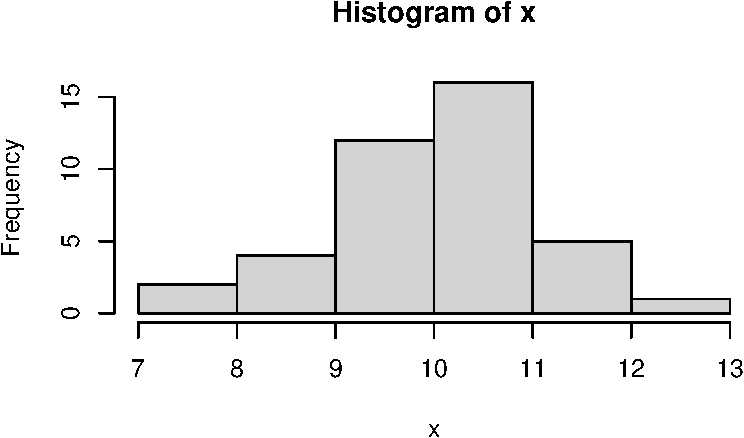
\includegraphics{0-R-tidyverse_files/figure-pdf/unnamed-chunk-18-1.pdf}

}

\end{figure}

\begin{Shaded}
\begin{Highlighting}[]
\FunctionTok{boxplot}\NormalTok{(x)}
\end{Highlighting}
\end{Shaded}

\begin{figure}[H]

{\centering 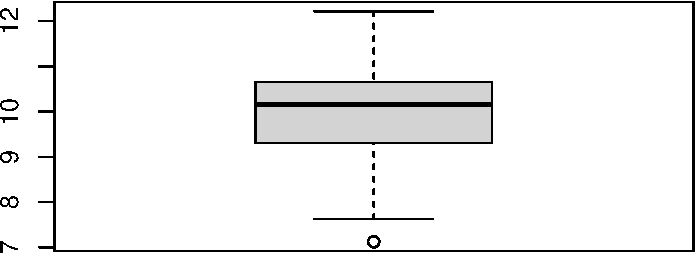
\includegraphics{0-R-tidyverse_files/figure-pdf/unnamed-chunk-18-2.pdf}

}

\end{figure}

\begin{Shaded}
\begin{Highlighting}[]
\FunctionTok{plot}\NormalTok{(x)}
\end{Highlighting}
\end{Shaded}

\begin{figure}[H]

{\centering 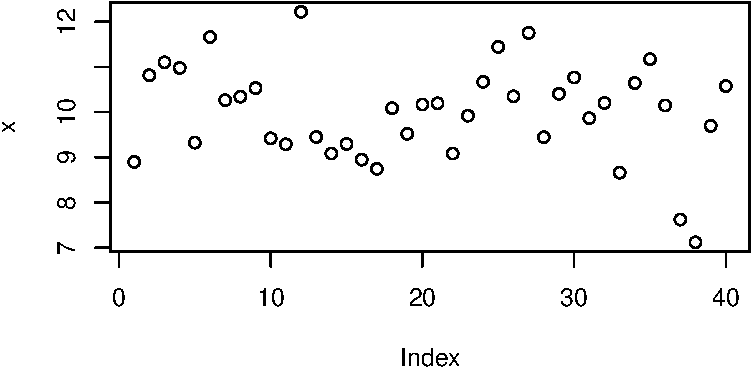
\includegraphics{0-R-tidyverse_files/figure-pdf/unnamed-chunk-18-3.pdf}

}

\end{figure}

\begin{Shaded}
\begin{Highlighting}[]
\FunctionTok{plot}\NormalTok{(}\FunctionTok{density}\NormalTok{(x), }\AttributeTok{xlab=}\StringTok{""}\NormalTok{)}
\end{Highlighting}
\end{Shaded}

\begin{figure}[H]

{\centering 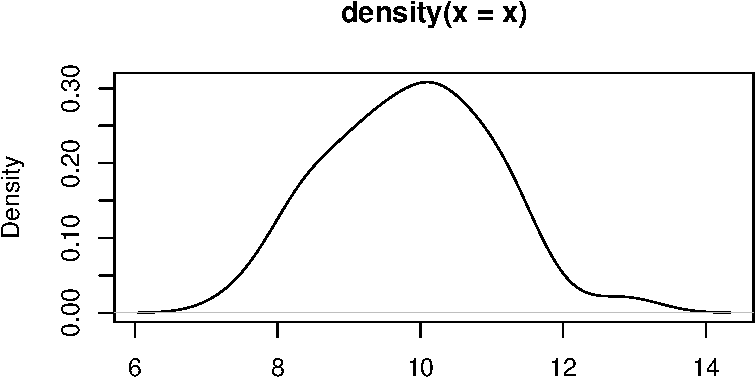
\includegraphics{0-R-tidyverse_files/figure-pdf/unnamed-chunk-18-4.pdf}

}

\end{figure}

\begin{Shaded}
\begin{Highlighting}[]
\FunctionTok{stripchart}\NormalTok{(}\FunctionTok{round}\NormalTok{(x,}\DecValTok{1}\NormalTok{), }\AttributeTok{method =} \StringTok{"stack"}\NormalTok{, }\AttributeTok{pch=}\DecValTok{20}\NormalTok{)}
\end{Highlighting}
\end{Shaded}

\begin{figure}[H]

{\centering 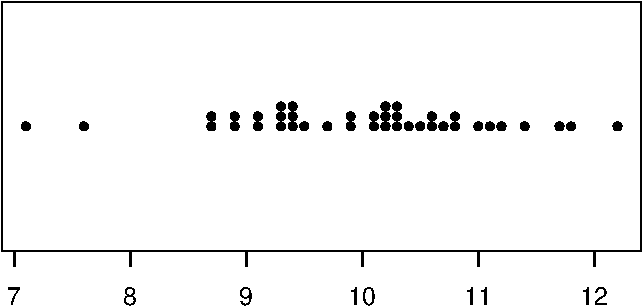
\includegraphics{0-R-tidyverse_files/figure-pdf/unnamed-chunk-18-5.pdf}

}

\end{figure}

\begin{Shaded}
\begin{Highlighting}[]
\FunctionTok{plot}\NormalTok{(}\FunctionTok{ecdf}\NormalTok{(x), }\AttributeTok{verticals=}\ConstantTok{TRUE}\NormalTok{)}
\end{Highlighting}
\end{Shaded}

\begin{figure}[H]

{\centering 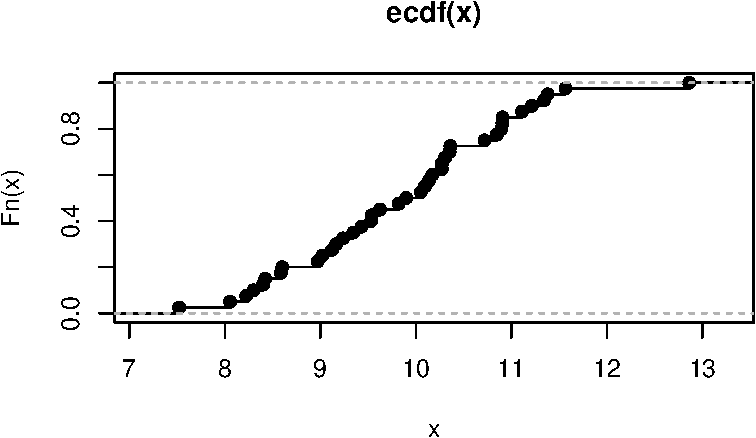
\includegraphics{0-R-tidyverse_files/figure-pdf/unnamed-chunk-18-6.pdf}

}

\end{figure}

We can form a matrix of order 3X2 or (or 2X3) and display all the above
six graphs in a panel. This is done using the option \texttt{par()},
which controls the graphics \emph{par}ameters.

\begin{Shaded}
\begin{Highlighting}[]
\NormalTok{x  }\OtherTok{\textless{}{-}} \FunctionTok{rnorm}\NormalTok{(}\DecValTok{40}\NormalTok{, }\DecValTok{10}\NormalTok{,}\DecValTok{1}\NormalTok{)}

\FunctionTok{par}\NormalTok{(}\AttributeTok{mfrow =} \FunctionTok{c}\NormalTok{(}\DecValTok{2}\NormalTok{, }\DecValTok{3}\NormalTok{))}

\FunctionTok{hist}\NormalTok{(x) }

\FunctionTok{boxplot}\NormalTok{(x)}

\FunctionTok{plot}\NormalTok{(x)}

\FunctionTok{plot}\NormalTok{(}\FunctionTok{density}\NormalTok{(x), }\AttributeTok{xlab=}\StringTok{\textquotesingle{}\textquotesingle{}}\NormalTok{)}

\FunctionTok{stripchart}\NormalTok{(}\FunctionTok{round}\NormalTok{(x,}\DecValTok{1}\NormalTok{), }\AttributeTok{method =} \StringTok{"stack"}\NormalTok{, }\AttributeTok{pch=}\DecValTok{20}\NormalTok{)}

\FunctionTok{plot}\NormalTok{(}\FunctionTok{ecdf}\NormalTok{(x), }\AttributeTok{verticals=}\ConstantTok{TRUE}\NormalTok{)}
\end{Highlighting}
\end{Shaded}

\begin{figure}[H]

{\centering 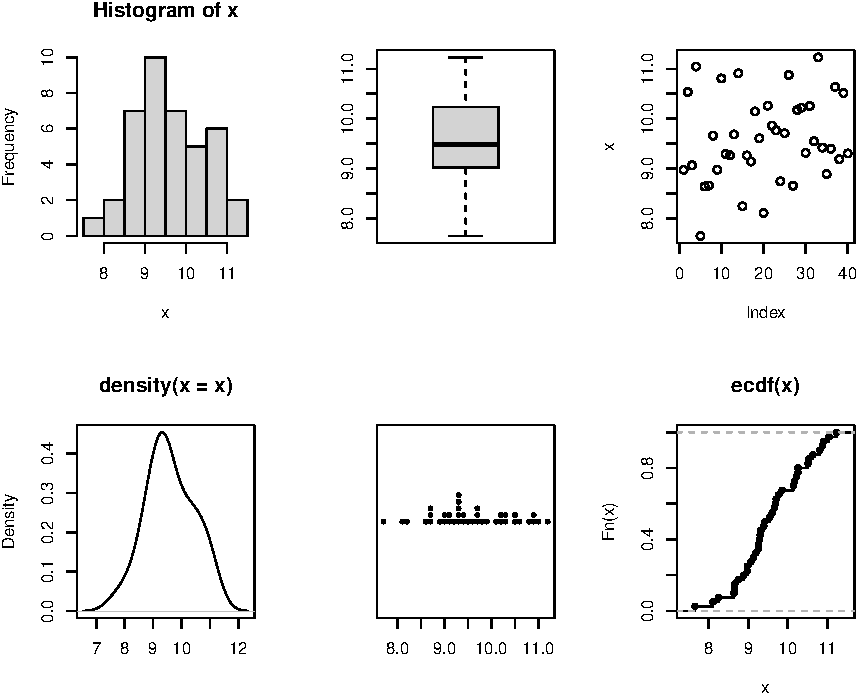
\includegraphics{0-R-tidyverse_files/figure-pdf/unnamed-chunk-19-1.pdf}

}

\end{figure}

Although we shall not cover them here, many plotting options can be set
using \texttt{par()} function; including size of margins, font types,
the colour of axis labels etc. See \texttt{help("par")}. The option
\texttt{par(new=T)} will be useful for an overlaid graph (instead of
splitting a graph). Try the following:

\begin{Shaded}
\begin{Highlighting}[]
\NormalTok{x  }\OtherTok{\textless{}{-}} \FunctionTok{rnorm}\NormalTok{(}\DecValTok{40}\NormalTok{, }\DecValTok{10}\NormalTok{,}\DecValTok{1}\NormalTok{)}

\FunctionTok{plot}\NormalTok{(x, }\AttributeTok{type =} \StringTok{"o"}\NormalTok{, }\AttributeTok{pch =} \DecValTok{1}\NormalTok{, }\AttributeTok{ylab =} \StringTok{""}\NormalTok{, }
     \AttributeTok{ylim =} \FunctionTok{c}\NormalTok{(}\FloatTok{6.5}\NormalTok{, }\FloatTok{13.5}\NormalTok{), }\AttributeTok{lty =} \DecValTok{1}\NormalTok{)}

\FunctionTok{par}\NormalTok{(}\AttributeTok{new=}\NormalTok{T)}

\NormalTok{y  }\OtherTok{\textless{}{-}}  \FunctionTok{rnorm}\NormalTok{(}\DecValTok{40}\NormalTok{, }\DecValTok{10}\NormalTok{,}\DecValTok{1}\NormalTok{)}

\FunctionTok{plot}\NormalTok{(y, }\AttributeTok{type =} \StringTok{"o"}\NormalTok{, }\AttributeTok{pch =} \DecValTok{2}\NormalTok{,}
     \AttributeTok{ylab =} \StringTok{"Two Batches of Random Normal Data"}\NormalTok{,}
     \AttributeTok{ylim =} \FunctionTok{c}\NormalTok{(}\FloatTok{6.5}\NormalTok{, }\FloatTok{13.5}\NormalTok{), }\AttributeTok{lty =} \DecValTok{2}\NormalTok{)}
\end{Highlighting}
\end{Shaded}

Note that \texttt{pch} specifies for the plotting character and
\texttt{lty} specifies the line type. You can add a legend by the
following command line:

\texttt{legend("topright",\ c("Batch\ I",\ "Batch\ II"),\ pch=1:2,\ lty=1:2)}

For scatter and other related plots, the command is \texttt{plot()}. Try

\begin{Shaded}
\begin{Highlighting}[]
\NormalTok{x  }\OtherTok{\textless{}{-}}  \FunctionTok{rnorm}\NormalTok{(}\DecValTok{40}\NormalTok{, }\DecValTok{10}\NormalTok{,}\DecValTok{1}\NormalTok{)}
\NormalTok{y  }\OtherTok{\textless{}{-}} \FunctionTok{rnorm}\NormalTok{(}\DecValTok{40}\NormalTok{, }\DecValTok{10}\NormalTok{,}\DecValTok{1}\NormalTok{)}
\FunctionTok{plot}\NormalTok{(y}\SpecialCharTok{\textasciitilde{}}\NormalTok{x)  }\CommentTok{\# or plot(x,y) }
\end{Highlighting}
\end{Shaded}

Add a title by the command

\texttt{title("This\ is\ my\ title")}

Add a reference line for the mean at the x-axis by the command

\texttt{abline(v=10)}

and again with \texttt{abline(h=10)} for the y-axis. A 45 degree (Y=X)
line can be added by the command

\texttt{abline(0,1)\ \#slope,\ b=1,\ y-intercept\ a=1}

You may also specify two points on the graph, and ask them to be
connected using the command

\texttt{lines(c(8,\ 12),\ c(8,\ 12),\ lty=2,\ col=4,\ lwd=2)}

Note that the \texttt{line()} has extra arguments to control the line
type, line width, and colour.

The command \texttt{rug(x)} draws will draw small vertical lines on the
x-axis (the command actually suits better for one dimensional graphs
such as a boxplot). Try

\texttt{rug(x)}

\texttt{rug(y,\ side=2)\ \ \#side\ =2\ specifies\ y-axis}

Graphs can be saved in various file formats, such as PDF (.pdf), JPEG
(.jpeg or .jpg), or postscript (.ps), by enclosing the plotting function
in the appropriate commands. For example, to save a simple figure as a
PDF file, we use the \texttt{pdf()} function.

\texttt{x\ \ \textless{}-\ \ 1:10}

\texttt{y\ \ \textless{}-\ \ x\^{}2}

\texttt{pdf(file\ =\ "Fig.pdf")}

\texttt{plot(x,\ y)}

\texttt{dev.off()}

The \texttt{command\ dev.off()} closes the file. You may use the copy
and paste facility for processing graphs or use the RStudio option to
save graphs.

The\texttt{lattice} package contains extra graphing facilities but such
graphs can be produced using \texttt{ggplot2} package. Try-

\begin{Shaded}
\begin{Highlighting}[]
\NormalTok{my.data }\OtherTok{\textless{}{-}}\FunctionTok{read.csv}\NormalTok{(}
  \StringTok{"https://www.massey.ac.nz/\textasciitilde{}anhsmith/data/tv.csv"}\NormalTok{, }
  \AttributeTok{header=}\ConstantTok{TRUE}\NormalTok{)}

\FunctionTok{library}\NormalTok{(lattice)}

\FunctionTok{bwplot}\NormalTok{(TELETIME }\SpecialCharTok{\textasciitilde{}} \FunctionTok{factor}\NormalTok{(SCHOOL), }
       \AttributeTok{data =}\NormalTok{ my.data)}
\end{Highlighting}
\end{Shaded}

\begin{figure}[H]

{\centering 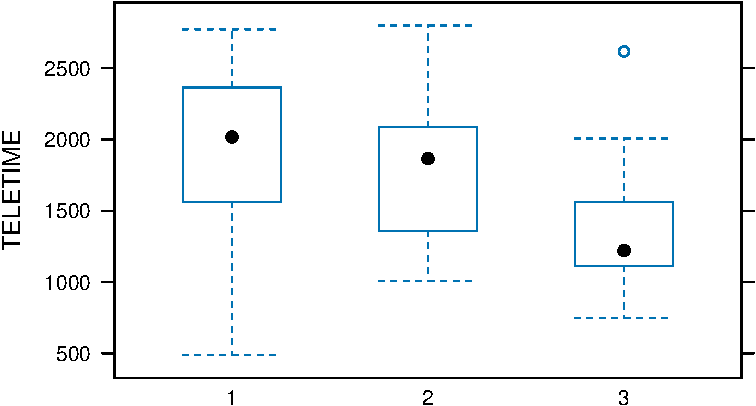
\includegraphics{0-R-tidyverse_files/figure-pdf/unnamed-chunk-22-1.pdf}

}

\end{figure}

It requires a bit of coding to combine base, lattice and ggplot graphs.
Try the following codes which combines three density plots of the same
data produced in different styles.

\begin{Shaded}
\begin{Highlighting}[]
\FunctionTok{library}\NormalTok{(}\StringTok{"grid"}\NormalTok{)}
\FunctionTok{library}\NormalTok{(}\StringTok{"ggplotify"}\NormalTok{)}

\NormalTok{x}\OtherTok{=} \FunctionTok{rnorm}\NormalTok{(}\DecValTok{30}\NormalTok{)}

\NormalTok{p1 }\OtherTok{\textless{}{-}} \FunctionTok{as.grob}\NormalTok{(}\SpecialCharTok{\textasciitilde{}}\FunctionTok{plot}\NormalTok{(}\FunctionTok{density}\NormalTok{(x)))}
\NormalTok{p1 }\OtherTok{\textless{}{-}} \FunctionTok{as.ggplot}\NormalTok{(p1)}

\NormalTok{p2 }\OtherTok{\textless{}{-}} \FunctionTok{as.grob}\NormalTok{(}\FunctionTok{densityplot}\NormalTok{(x))}
\NormalTok{p2 }\OtherTok{\textless{}{-}} \FunctionTok{as.ggplot}\NormalTok{(p2)}

\FunctionTok{library}\NormalTok{(ggplot2)}

\NormalTok{p3 }\OtherTok{\textless{}{-}} \FunctionTok{data.frame}\NormalTok{(}\AttributeTok{x=}\NormalTok{x) }\SpecialCharTok{|\textgreater{}} 
  \FunctionTok{ggplot}\NormalTok{() }\SpecialCharTok{+} 
  \FunctionTok{aes}\NormalTok{(x) }\SpecialCharTok{+}
  \FunctionTok{geom\_density}\NormalTok{()}

\FunctionTok{library}\NormalTok{(patchwork)}

\NormalTok{p1}\SpecialCharTok{/}\NormalTok{(p2}\SpecialCharTok{+}\NormalTok{p3)}
\end{Highlighting}
\end{Shaded}

\begin{tcolorbox}[enhanced jigsaw, colback=white, colframe=quarto-callout-tip-color-frame, breakable, rightrule=.15mm, title=\textcolor{quarto-callout-tip-color}{\faLightbulb}\hspace{0.5em}{Tip}, coltitle=black, titlerule=0mm, colbacktitle=quarto-callout-tip-color!10!white, leftrule=.75mm, bottomtitle=1mm, arc=.35mm, opacityback=0, toprule=.15mm, toptitle=1mm, opacitybacktitle=0.6, bottomrule=.15mm, left=2mm]

It is optional to work through the activities that follow to gain an
appreciation of how R works. Do not try to remember how to do everything
right now. For your assignment work, we will be given the R codes to
load data, graphing and modelling. These codes will give you a
head-start. Note that we often often learn R by doing and sometime
making mistakes.

\end{tcolorbox}

\emph{R default options for Hypothesis tests and modelling}

The \texttt{stats} default package in R has a number of functions for
performing hypothesis tests. However you will only use the following for
this course:

\texttt{ks.test} - Kolmogorov-Smirnov Tests

\texttt{shapiro.test} - Shapiro-Wilk Normality Test

\texttt{t.test} - Student's t-Test (one \& two samples, paired t-test
etc)

\texttt{pairwise.t.test} - Pairwise t tests (for multiple comparison)

\texttt{oneway.test} - Test for Equal Means in a One-Way Layout

\texttt{TukeyHSD} - To Compute Tukey's Honest Significant Differences

\texttt{var.test} - F Test to Compare Two Variances

\texttt{bartlett.test} - Bartlett Test of Homogeneity of Variances

\texttt{fisher.test} - Fisher's Exact Test for Count Data

\texttt{chisq.test} - Pearson's Chi-squared Test for Count Data

\texttt{cor.test} - Test for Association/Correlation Between Paired
Samples

The \texttt{car} package is needed for the following:

\texttt{durbinWatsonTest} Durbin-Watson Test for autocorrelated Errors

\texttt{leveneTest} Levene's Test

We will largely use the R function \texttt{lm} in this course. The
syntax for specifying a model under \texttt{lm} command (and various
other model related commands) is explained below:

The structure of the model is that the response variable is modelled as
a function of the response variables. The symbol
\texttt{\textasciitilde{}} (tilde) is used to say ``a function of''. The
simple regression of \texttt{y} on \texttt{x} is therefore specified as

\texttt{lm(y\ \textasciitilde{}\ x)}

The same applies to a one-way ANOVA in which \texttt{x} is a categorical
factor. For example, consider \texttt{tv.txt} dataset and the one-way
ANOVA model of \texttt{TELETIME} for \texttt{SCHOOL} is specified as
follows:

\begin{Shaded}
\begin{Highlighting}[]
\NormalTok{mydata }\OtherTok{\textless{}{-}} \FunctionTok{read.csv}\NormalTok{(}
  \StringTok{"https://www.massey.ac.nz/\textasciitilde{}anhsmith/data/tv.csv"}\NormalTok{, }
  \AttributeTok{header=}\ConstantTok{TRUE}
\NormalTok{  )}

\NormalTok{mymodel }\OtherTok{\textless{}{-}} \FunctionTok{lm}\NormalTok{(TELETIME }\SpecialCharTok{\textasciitilde{}} \FunctionTok{factor}\NormalTok{(SCHOOL), }
              \AttributeTok{data =}\NormalTok{ mydata) }\CommentTok{\# replace lm by aov and try}

\FunctionTok{summary}\NormalTok{(mymodel)}
\end{Highlighting}
\end{Shaded}

The function \texttt{summary()} gives the summary of the model (F
statistics, residual SD etc). The model summary output can be stored
into a text file using the function \texttt{sink()} or copy and paste in
the windows version. Graphs associated with a model can be obtained
using the command

\texttt{plot(mymodel)}

In the above context, we may also use the specific test command which
will give the same result but this test can also be performed without
assuming equal variances.

\begin{Shaded}
\begin{Highlighting}[]
\FunctionTok{oneway.test}\NormalTok{(TELETIME }\SpecialCharTok{\textasciitilde{}}\NormalTok{ SCHOOL, }
            \AttributeTok{var.equal =} \ConstantTok{TRUE}\NormalTok{, }
            \AttributeTok{data =}\NormalTok{ mydata) }
\end{Highlighting}
\end{Shaded}

For the \texttt{lm} command, note the following:

\texttt{+} indicates inclusion (not addition) of an explanatory variable
in the model

\texttt{-} indicates deletion (not subtraction) of an explanatory
variable from the model

\texttt{*} indicates the inclusion of the explanatory variables and
their interaction (not multiplication) between explanatory variables

\texttt{:} (colon) means only interaction between explanatory variables

\texttt{/} indicates the nesting (not division) of explanatory variables

\texttt{\textbar{}} indicates the conditioning (for example
\texttt{y\ \textasciitilde{}\ x\textbar{}z} means that y is a function
of x for given z).

For our course, you will not use the last two types. Some model examples
are given below:

\texttt{lm(y\ \textasciitilde{}\ x\ +\ z)} \#regression of y on x and z
(flat surface fit)

\texttt{lm(y\ \textasciitilde{}\ x*z)} \#includes the interaction term
ie \texttt{lm(y\ \textasciitilde{}\ x\ +\ z\ +\ x:z)}

\texttt{lm(y\ \textasciitilde{}\ x\ +\ I(x\^{}2)} \# fits a quadratic
model or use \texttt{poly(x,2)}

\texttt{lm(log(y)\ \textasciitilde{}\ sqrt(x)\ +\ log(z))} \#all
variables are transformed

As a further example, consider a study guide dataset. The following
commands fit a simple regression model and then plot the fitted line on
a scatter plot. Note that commands can be shortened but deliberately
shown this way.

\begin{Shaded}
\begin{Highlighting}[]
\NormalTok{mydata }\OtherTok{\textless{}{-}} \FunctionTok{read.csv}\NormalTok{(}
  \StringTok{"https://www.massey.ac.nz/\textasciitilde{}anhsmith/data/horsehearts.csv"}\NormalTok{, }
  \AttributeTok{header=}\ConstantTok{TRUE}
\NormalTok{  )}

\NormalTok{x }\OtherTok{\textless{}{-}}\NormalTok{ mydata}\SpecialCharTok{$}\NormalTok{EXTDIA}
\NormalTok{y }\OtherTok{\textless{}{-}}\NormalTok{ mydata}\SpecialCharTok{$}\NormalTok{WEIGHT}

\NormalTok{simplereg }\OtherTok{\textless{}{-}} \FunctionTok{lm}\NormalTok{(y }\SpecialCharTok{\textasciitilde{}}\NormalTok{ x)}
\end{Highlighting}
\end{Shaded}

Note that our model object \texttt{simplereg} can be queried in many
ways. The command \texttt{summary()} gives the following output.

\begin{Shaded}
\begin{Highlighting}[]
\FunctionTok{summary}\NormalTok{(simplereg)}
\CommentTok{\# or}
\CommentTok{\# library(broom)}
\CommentTok{\# tidy(simplereg)}
\CommentTok{\# glance(simplereg)}
\end{Highlighting}
\end{Shaded}

The command \texttt{names(simplereg)} will gives the names of many
individual components of the object \texttt{simplereg} we created. For
example, a plot of the residuals against the fitted values can be
obtained as

\begin{Shaded}
\begin{Highlighting}[]
\FunctionTok{plot}\NormalTok{(}\FunctionTok{residuals}\NormalTok{(simplereg) }\SpecialCharTok{\textasciitilde{}} \FunctionTok{fitted.values}\NormalTok{(simplereg))}
\end{Highlighting}
\end{Shaded}



\printbibliography


\end{document}
